\par Higgs particle has been the first fundamental scalar particle which was observed at LHC, CERN. Some years ago in 2012, both CMS and ATLAS collaborations announced its discovery ~\cite{Reference20,Reference21} with its mass around 125~GeV. Later on,
comprehensive properties of Higgs boson have been studied by these experiments~\cite{Reference22,Reference21a,Reference21b,Reference21c} which found to be compatible with SM Higgs boson. 
\par In this chapter, measurements of the fiducial cross sections (inclusive and differential) for the Higgs boson production in the $H \rightarrow 4\ell$ 
decay channel ($\ell = e, \mu$) with the full Run 2 proton-proton collisions of CMS at $\sqrt{s} = 13 TeV$ are presented which provide a direct test of perturbative QCD calculations of Standard Model (Higgs sector) at the TeV energy scale. Any deviation of the  integrated or  differential distributions from SM expectations would  provide a direct hint to BSM contributions. These measurements with earlier or partial Run2 CMS data has also been performed Ref. [JHEP 04 (2016) 005, CMSPAS HIG-15-004, JHEP 11 (2017) 047, HIG-17-028] . Nearly similar measurements have already been reported by ATLAS experiment 
in $H \rightarrow \gamma \gamma [ATLAS-CONF-2019-029] $~\cite{ATLAS:Hgg_8TeV,ATLAS:Hgg_8TeV_13TeV}, $H \rightarrow 4\ell$ [ATLAS-CONF-2019-025], ~\cite{ATLAS:H4l_8TeV,ATLAS:H4l_8TeV_13TeV} decay 
channels, combination of both channels [ATLAS-CONF-2019-032] ~\cite{ATLAS:H4l_Hgg_8TeV,ATLAS:H4l_Hgg_8TeV_13TeV} and by CMS experiment in $H \rightarrow \gamma \gamma$ decay 
channel~\cite{CMS:Hgg_8TeV}. 
\par The integrated fiducial cross section measurements 
are performed using collisions data corresponding to integrated luminosity of 137.1 $fb^{-1}$ at $\sqrt{s}=13$~TeV, recorded 
with the CMS detector at LHC. % 
To minimize the dependence of the results on the underlying models of the Higgs boson production  mechanism and  its properties, the cross sections are extracted in a fiducial phase space closely matching with the experimental acceptance as shown in Figure~\ref{fig:Models_cartoon}. The remaining model dependence is extracted by repeating the measurements for SM and other exotic models and reported as a distinct systematic uncertainty. All measurements includes the corrections for the finite detection efficiency and resolution effects. As $\sigma \times BR$ strongly depends on the Higgs mass, the measurements have been extracted assuming $m_H =  125.09$~GeV, as measured using the $H \rightarrow 2\gamma$ and $H \rightarrow 4\ell$
decay channels by the CMS experiment~\cite{Reference39}. 
%==================
\begin{figure}[!h!tb]
 \begin{center}
    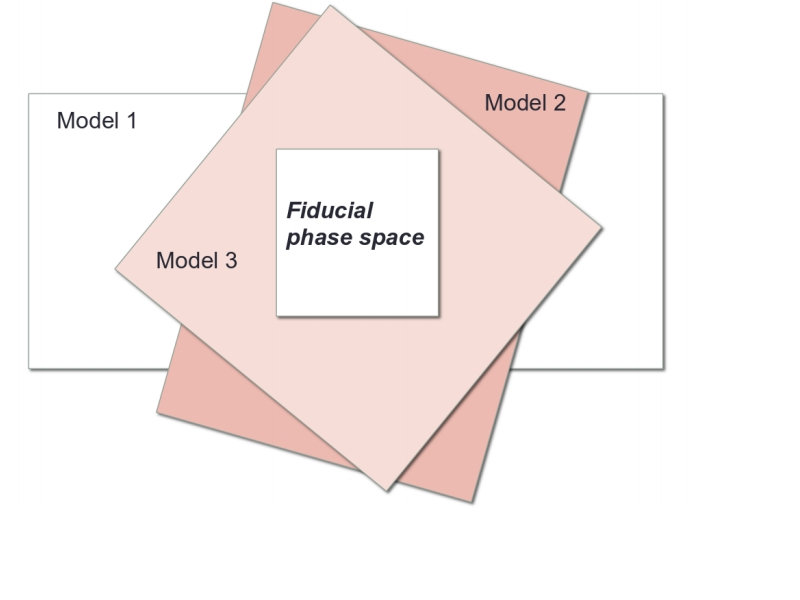
\includegraphics[width=0.65\textwidth,angle=0]{Figures/Models_cartoon.jpg}
    \caption{Fiducial phase definition among different models.}
 \label{fig:Models_cartoon}
 \end{center}
\end{figure}

%==================
\par The differential fiducial cross sections are measured as a function of %kinematic properties of the four-lepton system and the leading jet, as well as a 
%function of the jet multiplicity. The results are reported for 
 kinematic observables which are sensitive to the Higgs-boson production mechanisms: transverse momentum and the rapidity of the four-lepton 
system, transverse momentum of the leading jet and jet multiplicity.  

\par The chapter is structured as follows. The datasets and simulated samples used for the analysis are introduced in 
Section \ref{sec:DatasetsSimulation}. The analysis strategy is described in Section \ref{sec:AnalysisStrategy}, where fiducial phase space definition, 
event selection and method for extracting integrated and differential fiducial cross sections are explained.
In Section~\ref{sec:Systematics}  details of systematic uncertainties affecting the measurement are explained. In Section \ref{sec:Results} results 
are compared with SM theoretical predictions.  
